% !TeX root = surprises.tex

%%%%%%%%%%%%%%%%%%%%%%%%%%%%%%%%%%%%%%%%%%%%%%%%%%%%%%%%%%%%%%%%

\chapter{The Axioms of Origami}\label{c.origami-axioms}

%%%%%%%%%%%%%%%%%%%%%%%%%%%%%%%%%%%%%%%%%%%%%%%%%%%%%%%%%%%%%%%

\abstract*{Origami---the art of paper folding---was developed several centuries ago in Japan and now has a worldwide following. There is a mathematical theory of origami based on a set of seven axioms called the Huzita–Hatori axioms.
This chapter presents the axioms together with the equations of their folds and points of intersection using analytic geometry. The folds are also characterized as geometric loci.}

%%%%%%%%%%%%%%%%%%%%%%%%%%%%%%%%%%%%%%%%%%%%%%%%%%%%%%%%%%%%%%%

Origami, the art of paper folding, was developed several centuries ago in Japan and now has a worldwide following. In the late twentieth century the mathematical theory of origami was developed. Its foundation is a set of seven axioms, the 
\emph{Huzita–Hatori axioms}, named after Humiaki Huzita\index{Huzita, Humiaki} who formalized the first six axioms and Koshiro Hatori\index{Hatori, Koshiro} who found the seventh. Jacques Justin published all seven axioms several years before Huzita and Hatori, and Margherita P. Beloch\index{Beloch, Margherita P.} formulated the sixth axiom already in 1936. Nevertheless, the axioms as known as the Huzita-Hatori axioms.

In a series of three chapters we will explore the mathematics of origami. This chapter presents the axioms, Chap.~\ref{c.origami-cube} connects origami with the roots of polynomials and Chap.~\ref{c.origami-constructions} shows that constructions with origami can solve problems that are impossible using a straightedge and compass.
 
This chapter contains a section for each of the seven axioms. Following a statement of an axiom and a diagram of the \emph{fold} it specifies, the equations of the fold and the points of intersection are developed using analytic geometry. A fold can also be defined as a \emph{geometric locus}\index{Geometric locus}, the set of all points satisfying some property. The term fold comes from the origami operation of folding a piece of paper, but here it is used to refer the geometric line that would be created by folding the paper.

By definition folds result in \emph{reflections}\index{Origami!reflection}. Given a point $p$, its reflection around a fold $l$ results in a point $p'$, such that $l$ is the perpendicular bisector of the line segment $\overline{pp'}$ (Fig.~\ref{f.origami-def}).

\vspace{-2ex}

\begin{figure}[h]
\begin{center}
\begin{tikzpicture}[scale=.8]
\coordinate (P1) at (2,2);
\coordinate (P1P) at (6,4);
\coordinate (mid) at (4,3);
\draw[rotate=30] (mid) rectangle +(8pt,8pt);
\coordinate (m1) at ($(P1)!.5!(mid)$);
\coordinate (m2) at ($(mid)!.5!(P1P)$);
\draw[thick] (m1) -- +(120:4pt);
\draw[thick] (m1) -- +(-60:4pt);
\draw[thick] (m2) -- +(120:4pt);
\draw[thick] (m2) -- +(-60:4pt);
\draw[thick] (P1) -- (P1P);
\draw[very thick,dashed] (4.7,1.6) -- node[very near end,right,yshift=4pt] {$l$} (3.5,4);
\vertex{P1};
\vertex{P1P};
\node[above left] at (P1) {$p$};
\node[above left] at (P1P) {$p'$};
\draw[very thick,dotted,->,bend right=50] (2.1,1.9) to (6.05,3.9);
\end{tikzpicture}
\vspace{-2ex}
\end{center}
\caption{The fold is the perpendicular bisector of the line connecting a point and its reflection}\label{f.origami-def}
\end{figure}


\section{Axiom 1}\label{s.ax1}

\index{Origami!axiom 1}
\begin{axiom}
Given two distinct points $p_1=(x_1,y_1)$, $p_2=(x_2,y_2)$, there is a unique fold $l$ that passes through both of them (Fig.~\ref{f.origami-axiom1}).
\end{axiom}

\begin{figure}[ht]
\begin{center}
\begin{tikzpicture}[scale=1]
\draw[step=10mm,white!50!black,thin] (-1,-1) grid (8,6);
\draw[thick] (-1,0) -- (8,0);
\draw[thick] (0,-1) -- (0,6);
\foreach \x in {0,...,8}
  \node at (\x-.2,-.2) {\sm{\x}};
\foreach \y in {1,...,6}
  \node at (-.2,\y-.3) {\sm{\y}};
\coordinate (P1) at (2,2);
\coordinate (P2) at (6,4);
\draw[very thick,dashed] ($(P1)!-.75!(P2)$) -- node[very near end,below] {$l$} ($(P1)!1.5!(P2)$);
\vertex{P1};
\vertex{P2};
\node[above left] at (P1) {$p_1$};
\node[above left] at (P2) {$p_2$};

\draw[very thick,dotted,->,bend left=30] (2,5) to (4,1);
\end{tikzpicture}
\end{center}
\caption{Axiom $1$}\label{f.origami-axiom1}
\end{figure}

\noindent\textbf{Derivation of the equation of the fold:}
The equation of the fold $l$ is derived from the coordinates of $p_1$ and $p_2$. The slope is the quotient of the differences of the coordinates and the intercept is derived from $p_1$:
\begin{align}
y - y_1 = \frac{y_2-y_1}{x_2-x_1}(x-x_1)\,.
\end{align}

\begin{example}
Let  $p_1=(2,2), p_2=(6,4)$. The equation of $l$ is:
\begin{eqnarray*}
y-2&=&\frac{4-2}{6-2}(x-2)\\
y&=&\frac{1}{2}x+1\,.
\end{eqnarray*}
\end{example}

%%%%%%%%%%%%%%%%%%%%%%%%%%%%%%%%%%%%%%%%%%%%%%%%%%%%%%%%%%%%%%%%


\section{Axiom 2}\label{s.ax2}

\index{Origami!axiom 2}
\index{Origami!perpendicular bisector}
\begin{axiom}
Given two distinct points $p_1=(x_1,y_1)$, $p_2=(x_2,y_2)$, there is a unique fold $l$ that places $p_1$ onto $p_2$ (Fig.~\ref{f.origami-axiom2}).
\end{axiom}

The fold is the geometric locus of all points equidistant from $p_1$ and $p_2$.

\begin{figure}[ht]
\begin{center}
\begin{tikzpicture}[scale=1]
\draw[step=10mm,white!50!black,thin] (-1,-1) grid (8,6);
\draw[thick] (-1,0) -- (8,0);
\draw[thick] (0,-1) -- (0,6);
\foreach \x in {0,...,8}
  \node at (\x-.2,-.2) {\sm{\x}};
\foreach \y in {1,...,6}
  \node at (-.2,\y-.3) {\sm{\y}};
\coordinate (P1) at (2,2);
\coordinate (P2) at (6,4);
\coordinate (mid1) at ($(P1)!.5!(P2)$);
\coordinate (mid2) at ($(P1)!.5!(P2)+(-1,2)$);

\draw[rotate=30] (mid1) rectangle +(8pt,8pt);

\draw (P1) -- (P2);
\draw[very thick,dashed] ($(mid1)!-1.4!(mid2)$) -- node[very near end,left,yshift=-12pt] {$l$} ($(mid1)!1.4!(mid2)$);
\vertex{P1};
\vertex{P2};
\node[above left] at (P1) {$p_1$};
\node[above left] at (P2) {$p_2$};

\draw[very thick,dotted,->,bend right=50] (2.1,1.9) to (6,3.9);
\end{tikzpicture}
\end{center}
\caption{Axiom $2$}\label{f.origami-axiom2}
\end{figure}

\noindent\textbf{Derivation of the equation of the fold:}
The fold $l$ is the perpendicular bisector of $\overline{p_1p_2}$. Its slope is the negative reciprocal of the slope of the line connecting $p_1$ and $p_2$. $l$ passes through the midpoint between the points:
\begin{align}
y - \frac{y_1+y_2}{2} = -\frac{x_2-x_1}{y_2-y_1}\left(x-\frac{x_1+x_2}{2}\right)\,.\label{eq.midpoint1}
\end{align}

\begin{example}
Let $p_1=(2,2), p_2=(6,4)$. The equation of $l$ is:
%
\begin{eqnarray*}
y-\left(\frac{2+4}{2}\right)&=&-\frac{6-2}{4-2}\left(x-\left(\frac{2+6}{2}\right)\right)\\
y&=&-2x+11\,.
\end{eqnarray*}
\end{example}

%%%%%%%%%%%%%%%%%%%%%%%%%%%%%%%%%%%%%%%%%%%%%%%%%%%%%%%%%%%%%%%%


\section{Axiom 3}\label{s.ax3}

\index{Origami!axiom 3}
\begin{axiom}
Given two lines $l_1,l_2$, there is a fold $l$ that places $l_1$ onto $l_2$ (Fig.~\ref{f.origami-axiom3}).
\end{axiom}

The fold is the geometric locus of the points that are equidistant from $l_1$ and $l_2$, where the distance from a point to a line is the length of the line segment through the point that is perpendicular to the line. Using congruent triangles it is easy to show that the fold is a bisector of the angle formed by $l_1$ and $l_2$.

\begin{figure}[ht]
\begin{center}
\begin{tikzpicture}[scale=1]
\draw[step=10mm,white!50!black,thin] (-1,-1) grid (8,7);
\draw[thick] (-1,0) -- (8,0);
\draw[thick] (0,-1) -- (0,7);
\foreach \x in {0,...,8}
  \node at (\x-.2,-.2) {\sm{\x}};
\foreach \y in {1,...,7}
  \node at (-.2,\y-.3) {\sm{\y}};
\coordinate (L1a) at (2,2);
\coordinate (L1b) at (4,6);
\draw (L1a) -- node[very near start,right,yshift=-4pt] {$l_1$} (L1b);
\draw[name path=l1] ($(L1a)!-.75!(L1b)$) -- ($(L1a)!1.25!(L1b)$);
\coordinate (L2a) at (7,1);
\coordinate (L2b) at (4,4);
\draw (L2a) -- (L2b);
\draw[name path=l2] ($(L2a)!-.3!(L2b)$) -- node[very near start,above,xshift=4pt,yshift=2pt] {$l_2$} ($(L2a)!2!(L2b)$);
\path [name intersections = {of = l1 and l2, by = {PM}}];
\node[below left,xshift=-9pt,yshift=-7pt] at (PM) {$p_i$};

\node[above right,xshift=10pt,yshift=4pt] at (PM) {$\alpha$};
\node[below right,xshift=10pt] at (PM) {$\alpha$};
\node[above left,xshift=-3pt,yshift=12pt] at (PM) {$\beta$};
\node[above right,xshift=-3pt,yshift=12pt] at (PM) {$\beta$};

\coordinate (B1a) at (0,4.13);
\coordinate (B1b) at (6,5.1);
\draw[very thick,dashed] ($(B1a)!-.15!(B1b)$) -- node[very near start,above] {$l_{f_1}$}  ($(B1a)!1.35!(B1b)$);

\coordinate (B2a) at (3,6.73);
\coordinate (B2b) at (4,.57);
\draw[very thick,dashed] ($(B2a)!-.05!(B2b)$) -- node[very near end,right,xshift=4pt,yshift=6pt] {$l_{f_2}$} ($(B2a)!1.25!(B2b)$);

\draw[very thick,dotted,->,bend right=50] (6,2.2) to (4.5,6.7);
\draw[very thick,dotted,->,bend left=50] (6.2,1.6) to (1.8,1.3);
\end{tikzpicture}
\end{center}
\caption{Axiom $3$}\label{f.origami-axiom3}
\end{figure}

\noindent\textbf{Derivation of the equation of the fold:}

If the lines are parallel, let $l_1$ be $y=mx+b_1$ and let $l_2$ be $y=mx+b_2$. The fold is the line parallel to $l_1$ and $l_2$ that is halfway between them:
\[
y=mx+\frac{b_1+b_2}{2}\,.
\]

If the lines intersect, let $l_1$ be $y=m_1x+b_1$ and let $l_2$ be $y=m_2x+b_2$.
$p_i=(x_i,y_i)$, the point of intersection of the two lines, is:
%
\begin{eqnarray*}
m_1x_i+b_1&=&m_2x_i+b_2\\
x_i &=& \frac{b_2-b_1}{m_1-m_2}\\
y_i &=&m_1x_i+b_1\,.
\end{eqnarray*}

\begin{example}\label{ex.axiom3}
Let $l_1$ be $y=2x-2$ and let $l_2$ be $y=-x+8$. Then $p_i=(x_i,y_i)$ is:
\begin{eqnarray*}
x_i&=&\frac{8-(-2)}{2-(-1)}=\frac{10}{3}\approx 3.33\\
y_i &=& 2\cdot\frac{10}{3}-2=\frac{14}{3}\approx 4.67\,.
\end{eqnarray*}
\end{example}

\index{Origami!angle bisector}
The fold is the bisector of the angle formed by $l_1$ and $l_2$ at their point of intersection. There are two possible folds since there are two pairs of vertical angles. We need to determine the slopes of the angle bisectors. If the angle of line $l_1$ relative to the $x$-axis is $\theta_1$ and the angle of line $l_2$ relative to the $x$-axis is $\theta_2$, then the fold is the line which makes an angle of $\theta_b=(\theta_1+\theta_2)/2$ relative to the $x$-axis.

Let $m_1=\tan\theta_1, m_2=\tan \theta_2$. By Thm.~\ref{thm.tangent-sum}, $m_s$, the slope of the line making an angle of $\theta_1+\theta_2$ relative to the $x$-axis, is:
\[
m_s=\tan(\theta_1+\theta_2)= \frac{\tan\theta_1+\tan\theta_2}{1-\tan\theta_1\tan\theta_2}=\frac{m_1+m_2}{1-m_1m_2}\,.
\]
By Thm.~\ref{thm.tangent-half}, $m_b$, the slope of the angle bisector, is:
\[
m_b= \tan\frac{\theta_1+\theta_2}{2}=\frac{-1\pm\sqrt{1+\tan^2(\theta_1+\theta_2)}}{\tan (\theta_1+\theta_2)}=\frac{-1\pm\sqrt{1+m_s^2}}{m_s}\,.
\]
\begin{example}
For $y=2x-2$ and $y=-x+8$, the slope of the angle bisector is:
%
\begin{eqnarray*}
m_s&=&\frac{2+(-1)}{1-(2 \cdot -1)}=\frac{1}{3}\\
m_b&=&\frac{-1\pm\sqrt{1+(1/3)^2}}{1/3}=-3\pm \sqrt{10}\approx -6.16,\; 0.162\,.
\end{eqnarray*}
\end{example}

Let us derive the equation of the fold $l_{f_1}$ with the positive slope. From Example~\ref{ex.axiom3}, the coordinates of the intersection of the two lines are $(10/3, 14/3)$. Therefore:
\begin{eqnarray*}
\frac{14}{3} &=& (-3+\sqrt{10}) \cdot \frac{10}{3} + b_i\\ b_i&=&\frac{44-10\sqrt{10}}{3}\\
y&=& (-3+\sqrt{10})x + \frac{44-10\sqrt{10}}{3}\approx 0.162x+4.13\,.
\end{eqnarray*}

%%%%%%%%%%%%%%%%%%%%%%%%%%%%%%%%%%%%%%%%%%%%%%%%%%%%%%%%%%%%%%%%


\section{Axiom 4}\label{s.ax4}

\index{Origami!axiom 4}
\begin{axiom}
Given a point $p_1$ and a line $l_1$, there is a unique fold $l$ perpendicular to $l_1$ that passes through point $p_1$ (Fig.~\ref{f.origami-axiom4}).
\end{axiom}

The fold is the geometric locus of all points on the line perpendicular to $l_1$ that passes through $p_1$.

\begin{figure}[ht]
\begin{center}
\begin{tikzpicture}[scale=1]
\draw[step=10mm,white!50!black,thin] (-1,-1) grid (8,7);
\draw[thick] (-1,0) -- (8,0);
\draw[thick] (0,-1) -- (0,7);
\foreach \x in {0,...,8}
  \node at (\x-.2,-.2) {\sm{\x}};
\foreach \y in {1,...,7}
  \node at (-.2,\y-.3) {\sm{\y}};
\coordinate (L1a) at (2,0);
\coordinate (L1b) at (5,6);
\draw (L1a) -- node[very near start,right,yshift=-4pt] {$l_1$} ($(L1a)!1.15!(L1b)$);
\coordinate (P1) at (2,6);
\vertex{P1};
\node[above right] at (P1) {$p_1$};
\draw[thick,dashed] (0,7) -- node[very near end,above right] {$l$} (8,3);
\coordinate (intersection) at (4.4,4.8);
\draw[rotate=-30] (intersection) rectangle +(8pt,8pt);

\draw[very thick,dotted,->,bend left=50] (5.4,6.3) to (3.7,3);
\end{tikzpicture}
\end{center}
\caption{Axiom $4$}\label{f.origami-axiom4}
\end{figure}

\noindent\textbf{Derivation of the equation of the fold:}
Let $l_1$ be $y = m_1x + b_1$ and let $p_1=(x_1,y_1)$.  $l$ is perpendicular to $l_1$ so its slope is $-(1/m_1)$. Since it passes through $p_1$, we can compute the intercept $b$ and write down its equation:
%
\begin{eqnarray*}
y_1&=&-\frac{1}{m} x_1 + b\\
b&=& \frac{(my_1+x_1)}{m}\\
y&=&-\frac{1}{m} x +\frac{(my_1+x_1)}{m}\,.
\end{eqnarray*}
\begin{example}
Let $p_1=(2,6)$ and let $l_1$ be $y=2x-4$. The equation of the fold $l$ is:
\[
y=-\frac{1}{2}x + \frac{2\cdot 6 + 2}{2}=-\frac{1}{2}x + 7\,.
\]
\end{example}


%%%%%%%%%%%%%%%%%%%%%%%%%%%%%%%%%%%%%%%%%%%%%%%%%%%%%%%%%%%%%%%%


\section{Axiom 5}\label{s.ax5}

\index{Origami!axiom 5}
\begin{axiom}
Given two points $p_1,p_2$ and a line $l_1$, there is a fold $l$ that places $p_1$ onto $l_1$ and passes through $p_2$ (Fig.~\ref{f.origami-axiom5}).
\end{axiom}

The geometric locus of the reflection of $p_1$ is the circle centered at $p_2$ with radius $\overline{p_1p_2}$, since the fold passes through $p_2$ and $p_2$ is on the perpendicular bisector of $\overline{p_1p_1'}$. The fold is constrained so that  the reflection $p_1'$ is on the given line $l_1$.

\begin{figure}[ht]
\begin{center}
\begin{tikzpicture}[scale=1]
\draw[step=10mm,white!50!black,thin] (-1,-1) grid (9,9);
\draw[thick] (-1,0) -- (9,0);
\draw[thick] (0,-1) -- (0,9);
\foreach \x in {0,...,9}
  \node at (\x-.2,-.2) {\sm{\x}};
\foreach \y in {1,...,9}
  \node at (-.2,\y-.3) {\sm{\y}};
\coordinate (L1a) at (0,3);
\coordinate (L1b) at (8,-1);
\draw (L1a) -- node[near end,below right,xshift=8pt,yshift=-8pt] {$l_1$} (L1b);
\coordinate (P1) at (2,8);
\coordinate (P2) at (4,4);
\vertex{P1};
\vertex{P2};
\node[above left] at (P1) {$p_1$};
\node[above left,yshift=4pt] at (P2) {$p_2$};


\draw[name path=L1] (8,-1) -- (-1,3.5);
\node[draw,name path = circle] at (P2)
    [circle through = (P1)] {};

\path [name intersections = {of = circle and L1, by = {P1P,P1PP}}];
\vertex{P1P};
\vertex{P1PP};
\node[above left,xshift=-2pt,yshift=4pt] at (P1P) {$p_1'$};
\node[above left,yshift=6pt] at (P1PP) {$p_1''$};

\coordinate (f1) at (0,6);
\draw[thick,dashed] ($(f1)!-.25!(P2)$) -- node[very near end,above] {$l_{f_2}$} ($(f1)!2.25!(P2)$);
\coordinate (f2) at (0,2);
\draw[thick,dashed] ($(f2)!-.25!(P2)$) -- node[very near end,below,yshift=-2pt] {$l_{f_1}$} ($(f2)!2.25!(P2)$);

\draw[very thick,dotted,->,bend left=50] (2.1,7.9) to (-.3,3.2);
\draw[very thick,dotted,->,bend left=50] (2.2,7.95) to (6.05,.1);
\end{tikzpicture}
\end{center}
\caption{Axiom $5$}\label{f.origami-axiom5}
\end{figure}

\noindent\textbf{Derivation of the equations of the folds:}
Let $l_1$ be $y=m_1x + b_1$ and let $p_1=(x_1,y_1)$, $p_2=(x_2,y_2)$. The equation of the circle centered at $p_2$ with radius $\overline{p_1p_2}$ is:
\begin{eqnarray*}
(x-x_2)^2 + (y-y_2)^2 = r^2\,,\quad \textrm{where}\\
r^2= (x_2-x_1)^2 + (y_2-y_1)^2\,.
\end{eqnarray*}

\newpage

Substituting the equation of $l_1$ into the equation for the circle gives:
\begin{eqnarray*}
(x-x_2)^2+((m_1x+b_1)-y_2)^2&=&r^2\\
(x-x_2)^2+(m_1x+(b_1-y_2))^2&=&r^2\,,
\end{eqnarray*}
and we obtain a quadratic equation for the $x$-coordinates of the possible intersections:
\begin{align}
x^2(1+m_1^2) \,+\, 2(-x_2+m_1(b-y_2))x \,+\,(x_2^2 + (b_1^2 - 2b_1y_2+y_2^2)-r^2)=0\,.\label{eq.intersections}
\end{align}
Since the quadratic equation has at most two solutions for a given pair of points and a line, there may be zero, one or two folds. From the solutions $x_1',x_1''$, we can compute $y_1',y_1''$ from $y=m_1x+b_1$. The reflected points are $p_1'=(x_1',y_1')$, $p_1''=(x_1'',y_1'')$.
\begin{example}
Let $p_1=(2,8)$, $p_2=(4,4)$ and let $l_1$ be $y=-\frac{1}{2}x +3$. The equation of the circle is $(x-4)^2 + (y-4)^2 = (4-2)^2+(4-8)^2=20$.

Substitute the equation of the line into the equation of the circle to obtain a quadratic equation for the $x$-coordinates of the intersections (or use Eq.~\ref{eq.intersections}):
\begin{eqnarray*}
(x-4)^2 + \left(\left(-\frac{1}{2}x+3\right)-4\right)^2&=&20\\
(x-4)^2 + (-1)^2\cdot\left(\frac{1}{2}x+1\right)^2-20&=&0\\
5x^2 -28x -12&=&0\\
(5x+2)(x-6)&=&0\,.
\end{eqnarray*}
The two points of intersection are:
\[
p_1'=(-2/5,16/5) = (-0.4,3.2)\,,\quad p_1''=(6,0)\,.
\]
\end{example}
The folds will be the perpendicular bisectors of $\overline{p_1p_1'}$ and $\overline{p_1p_1''}$.
\begin{example}
For $p_1=(2,8)$ and $p_1'=(-2/5,16/5)$ the equation of $l_{f_1}$  is:
\begin{eqnarray*}
y-\frac{8+(16/5)}{2}&=&-\frac{(-2/5)-2}{(16/5)-8}\left(x-\frac{2+\left(-2/5\right)}{2}\right)\\
y&=&-\frac{1}{2}x+6\,.
\end{eqnarray*}
\end{example}

\begin{example}
For $p_1=(2,8)$ and $p_1''=(6,0)$ the equation of the fold $l_{f_2}$ is:
%
\begin{eqnarray*}
y-\frac{8+0}{2}&=&-\frac{6-2}{0-8}\left(x-\frac{2+6}{2}\right)\\
y&=&\frac{1}{2}x+2\,.
\end{eqnarray*}
\end{example}

%%%%%%%%%%%%%%%%%%%%%%%%%%%%%%%%%%%%%%%%%%%%%%%%%%%%%%%%%%%%%%%%



\section{Axiom 6}\label{s.ax6}
\index{Origami!axiom 6}
\begin{axiom}
Given two points $p_1,p_2$ and two lines $l_1,l_2$, there is a fold $l$ that places $p_1$ onto $l_1$ and places $p_2$ onto $l_2$ (Fig.~\ref{f.origami-axiom6}).
\end{axiom}

A fold that places $p_i$ onto $l_i$ is a line $l_f$ such that the distance from $p_i$ to $l_f$ is equal to the distance from $l_i$ to $l_f$. The geometric locus of points equidistant from a point $p_i$ and a line $l_i$ is a \emph{parabola}. $p_i$ is called the \emph{focus}\index{Focus of a parabola} and $l_1$ is called the \emph{directrix}\index{Directrix of a parabola}.\index{Parabola!locus@as the locus of a fold} A fold is any line tangent to the parabola (Sect.~\ref{s.parabola}).

\begin{figure}[ht]
\begin{center}
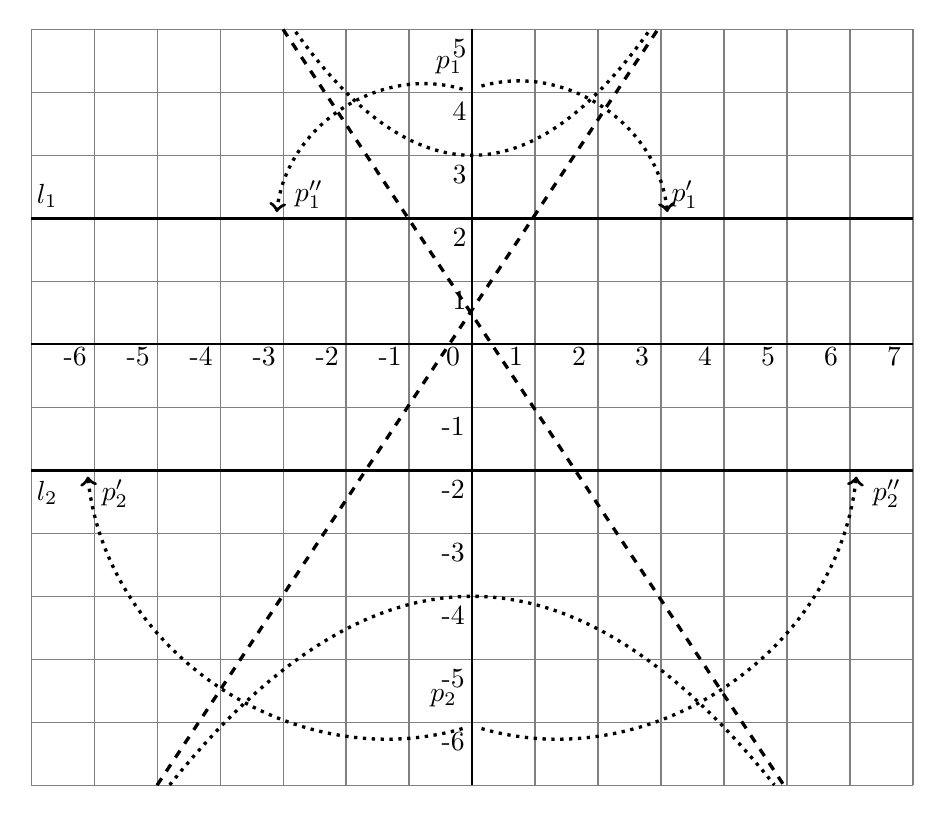
\begin{tikzpicture}[scale=.8]
\draw[step=10mm,white!50!black,thin] (-7,-7) grid (7,5);
\draw[thick] (-7,0) -- (7,0);
\draw[thick] (0,-7) -- (0,5);
\foreach \x in {-6,...,7}
  \node at (\x-.3,-.2) {\sm{\x}};
\foreach \y in {1,...,5}
  \node at (-.2,\y-.3) {\sm{\y}};
\foreach \y in {-6,...,-1}
  \node at (-.3,\y-.3) {\sm{\y}};
  
\coordinate (P1) at (0,4);
\coordinate (P2) at (0,-6);
\coordinate (P1P) at (3.1,2);
\coordinate (P2P) at (-6.12,-2);
\coordinate (P1PP) at (-3.1,2);
\coordinate (P2PP) at (6.12,-2);

\vertex{P1};
\vertex{P2};
\vertex{P1P};
\vertex{P2P};
\vertex{P1PP};
\vertex{P2PP};

\node[above left,yshift=3pt] at (P1) {$p_1$};
\node[above left,xshift=-2pt,yshift=2pt] at (P2) {$p_2$};
\node[above right,xshift=-2pt] at (P1P) {$p_1'$};
\node[below right,xshift=2pt] at (P2P) {$p_2'$};
\node[above right,xshift=3pt] at (P1PP) {$p_1''$};
\node[below right,xshift=2pt] at (P2PP) {$p_2''$};

\draw[very thick] (-7,2) -- node[very near start,above,xshift=-34pt] {$l_1$} (7,2);
\draw[very thick] (-7,-2) -- node[very near start,below,xshift=-34pt] {$l_2$} (7,-2);

\draw[domain=-4.8:4.8,samples=50,very thick,dotted] plot (\x,{-.13*\x*\x-4});
\draw[domain=-2.8:2.8,samples=50,very thick,dotted] plot (\x,{.25*\x*\x+3});

\draw[very thick,dashed] (-5,-7) -- (2.95,5);
\draw[very thick,dashed] (-3,5) -- (4.95,-7);

\draw[very thick,dotted,->,bend left=50] (.15,4.1) to (3.1,2.1);
\draw[very thick,dotted,->,bend right=50] (-.15,4.05) to (-3.1,2.1);

\draw[very thick,dotted,->,bend right=50] (.15,-6.1) to (6.1,-2.1);
\draw[very thick,dotted,->,bend left=50] (-.15,-6.1) to (-6.1,-2.1);

\end{tikzpicture}
\end{center}
\caption{Axiom $6$}\label{f.origami-axiom6}
\end{figure}

For a fold to simultaneously place $p_1$ onto $l_1$ and $p_2$ onto $l_2$, it must be a tangent common to the two parabolas. There may be zero, one, two or three common tangents (Figs.~\ref{f.two-para-1-zero}, \ref{f.two-para-1-one}, \ref{f.two-para-1-two}, \ref{f.two-para-1-three}).\index{Parabola!common tangents to two parabolas}
\begin{figure}[ht]
\subfigures
\leftfigure[c]{
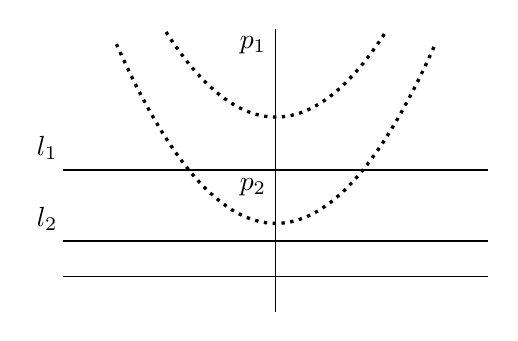
\begin{tikzpicture}[scale=.45]
\draw (-6,0) -- (6,0);
\draw (0,-1) -- (0,7);
\coordinate (P1) at (0,6);
\coordinate (P2) at (0,2);
\vertex{P1};
\vertex{P2};
\node[above left] at (P1) {$p_1$};
\node[above left] at (P2) {$p_2$};
\draw[thick] (-6,3) -- node[very near start,above,xshift=-25pt] {$l_1$} (6,3);
\draw[thick] (-6,1) -- node[very near start,above,xshift=-25pt] {$l_2$} (6,1);
\draw[domain=-3.1:3.1,samples=50,very thick,dotted] plot (\x,{.25*\x*\x+4.5});
\draw[domain=-4.5:4.5,samples=50,very thick,dotted] plot (\x,{.25*\x*\x+1.5});
\end{tikzpicture}
}
\hfill
\rightfigure[c]{
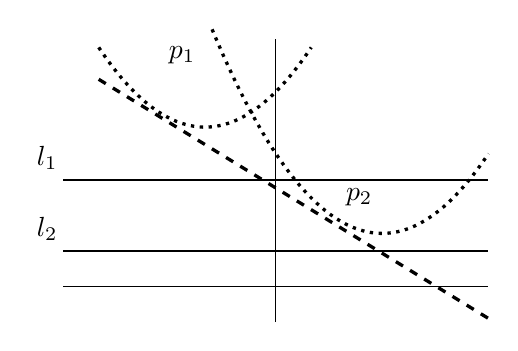
\begin{tikzpicture}[scale=.45]
\draw (-6,0) -- (6,0);
\draw (0,-1) -- (0,7);
\coordinate (P1) at (-2,6);
\coordinate (P2) at (3,2);
\vertex{P1};
\vertex{P2};
\node[above left] at (P1) {$p_1$};
\node[above left] at (P2) {$p_2$};
\draw[thick] (-6,3) -- node[very near start,above,xshift=-25pt] {$l_1$} (6,3);
\draw[thick] (-6,1) -- node[very near start,above,xshift=-25pt] {$l_2$} (6,1);
\draw[domain=-5:1,samples=50,very thick,dotted] plot (\x,{.25*(\x+2)*(\x+2)+4.5});
\draw[domain=-1.8:6,samples=50,very thick,dotted] plot (\x,{.25*(\x-3)*(\x-3)+1.5});
\draw[very thick,dashed] (-5,5.85) -- (6,-.9);
\end{tikzpicture}
}
\leftcaption{No common tangents}\label{f.two-para-1-zero}
\rightcaption{One common tangent}\label{f.two-para-1-one}
\end{figure}


\begin{figure}[ht]
\subfigures
\leftfigure[c]{
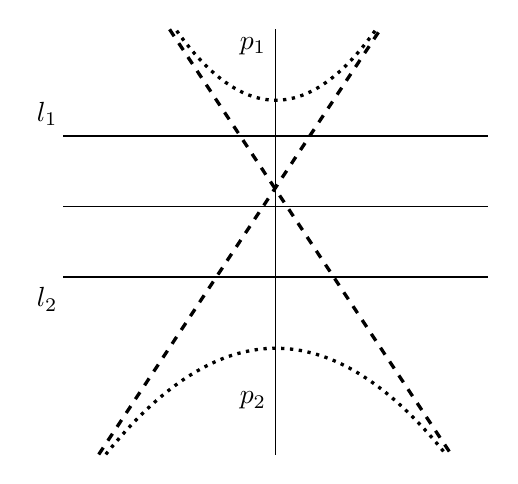
\begin{tikzpicture}[scale=.45]
\draw (-6,0) -- (6,0);
\draw (0,-7) -- (0,5);
\coordinate (P1) at (0,4);
\coordinate (P2) at (0,-6);
\vertex{P1};
\vertex{P2};
\node[above left] at (P1) {$p_1$};
\node[above left] at (P2) {$p_2$};
\draw[thick] (-6,2) -- node[very near start,above,xshift=-25pt] {$l_1$} (6,2);
\draw[thick] (-6,-2) -- node[very near start,below,xshift=-25pt] {$l_2$} (6,-2);
\draw[domain=-4.8:4.8,samples=50,very thick,dotted] plot (\x,{-.13*\x*\x-4});
\draw[domain=-2.8:2.8,samples=50,very thick,dotted] plot (\x,{.25*\x*\x+3});
\draw[very thick,dashed] (-5,-7) -- (2.95,5);
\draw[very thick,dashed] (-3,5) -- (4.95,-7);
\end{tikzpicture}
}
\hfill
\rightfigure[c]{
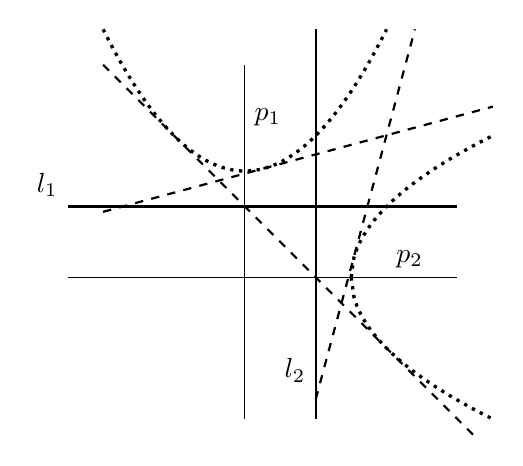
\begin{tikzpicture}[scale=.45]
\draw (-5,0) -- (6,0);
\draw (0,-4) -- (0,6);
\coordinate (P1) at (0,4);
\coordinate (P2) at (4,0);
\vertex{P1};
\vertex{P2};
\node[above right] at (P1) {$p_1$};
\node[above right] at (P2) {$p_2$};
\draw[thick] (-5,2) -- node[very near start,above,xshift=-25pt] {$l_1$} (6,2);
\draw[thick] (2,-4) -- node[very near start,left] {$l_2$} (2,7);
\draw[domain=-4:4,samples=50,very thick,dotted] plot (\x,{.25*\x*\x+3});
\draw[domain=3:7,samples=50,very thick,dotted] plot (\x,{sqrt(4*\x-12)});
\draw[domain=3:7,samples=50,very thick,dotted] plot (\x,{-sqrt(4*\x-12)});

\draw[thick,dashed,domain=-4:6.5] plot (\x,-\x+2);
\draw[thick,dashed,domain=-4:7] plot (\x,.27*\x+2.93);
\draw[thick,dashed,domain=2:4.8] plot (\x,3.73*\x-10.9);
\end{tikzpicture}
}
\leftcaption{Two common tangents}\label{f.two-para-1-two}
\rightcaption{Three common tangents}\label{f.two-para-1-three}
\end{figure}

The formula for an arbitrary parabola is quite complex, so we limit the presentation to parabolas whose axis of symmetry is the $y$-axis.

\subsection{Derivation of the Equation of a Fold}

Let $(0,f)$ be the focus of a parabola with directrix $y=d$. Define $p=f-d$, the signed length of the line segment between the focus and the directrix.\footnote{We have been using the notation $p_i$ for points; the use of $p$ here might be confusing but it is the standard notation. The formal name for $p$ is one-half the \emph{latus rectum}.} If the vertex of the parabola is on the $x$-axis, the equation of the parabola is $y=x^2/2p$. To move the parabola up or down the $y$-axis so that its vertex is at $(0,h)$, add $h$ to the equation of the parabola (Fig.~\ref{f.elements-parabola}):
\[y=\frac{x^2}{2p}+h\,.\]

\begin{figure}[htb]
\begin{center}
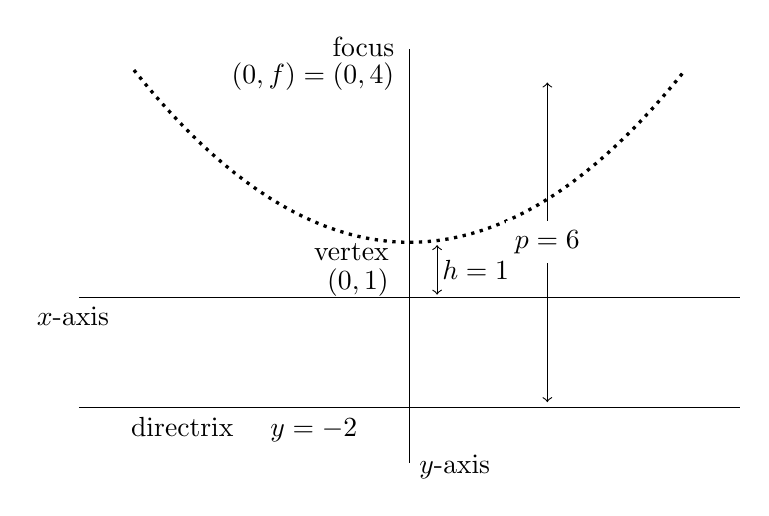
\begin{tikzpicture}[scale=.7]
\draw (-6,0) -- node[very near start,below,xshift=-32pt] {$x$-\textrm{axis}}(6,0);
\draw (0,-3) -- node[very near start,right,yshift=-20pt] {$y$-\textrm{axis}}(0,4.5);
\draw (-6,-2) -- node[near start,below] {\textrm{directrix} $\quad y=-2$} (6,-2);
\draw[domain=-5:5,samples=50,very thick,dotted] plot (\x,{\x*\x/8+1});
\coordinate (F) at (0,4);
\coordinate (V) at (0,1);
\coordinate (Y) at (0,-2);
\vertex{F};
\node[left,xshift=-2pt,yshift=0pt] at (F) {$(0,f)=(0,4)$}; \node[above left,xshift=-2pt,yshift=4pt] at (F) {\textrm{focus}};
\node[below left,xshift=-4,yshift=3pt] at (V) {\textrm{vertex}};
\node[below left,xshift=-4,yshift=-6pt] at (V) {$(0,1)$};
\draw[<->] (2.5,-1.9) -- node[fill=white] {$p=6$} +(0,5.8);
\draw[<->] (.5,.05) -- +(0,.9);
\node at (1.2,.5) {$h=1$} +(0,.9);
\end{tikzpicture}
\end{center}
\caption{The elements in the definition of a parabola}\label{f.elements-parabola}
\end{figure}

\newpage

Define $a=2ph$ so that the equation of the parabola is:
\begin{subeqnarray}
y&=&\frac{x^2}{2p}+\frac{a}{2p}\\
x^2-2py+a&=&0\,.\slabel{eq.eq-parabola}
\end{subeqnarray}
The equation of the parabola in Fig.~\ref{f.elements-parabola} is $x^2-12y +12=0$.

Substitute the equation of an \emph{arbitrary} line $y=mx+b$ into Eq.~\ref{eq.eq-parabola} to obtain an equation for the points of intersection of the line and the parabola:
\begin{eqnarray*}
x^2-2p(mx+b)+a&=&0\\
x^2+(-2mp)x+(-2pb+a)&=&0\,.
\end{eqnarray*}
The line will be tangent to the parabola if and only if this quadratic equation has \emph{exactly one solution} if and only if its discriminant is zero:
\begin{subeqnarray}
(-2mp)^2\:-\:4\cdot 1\cdot (-2pb+a)=0\\
m^2p^2+2pb-a=0\,.\slabel{eq.disc}
\end{subeqnarray}

This is an equation with variables $m,b$ for the tangents to the parabola. To obtain the common tangents to both parabolas, the equations for the two parabolas have two unknowns and can be solved for $m$ and $b$.

\newpage

\begin{example}\mbox{}

\noindent\textbf{Parabola 1:} Focus $(0,4)$, directrix $y=2$, vertex $(0,3)$.

\noindent{}$p=2$, $a=2\cdot 2\cdot 3=12$. The equation of the parabola is:
\[
x^2-4y +12=0\,.
\]
Substituting $p$ and $a$ into Eq.~\ref{eq.disc} and simplifying gives:
\[
m^2+b-3=0\,.
\]

\noindent\textbf{Parabola 2:} Focus $(0,-4)$, directrix $y=-2$, vertex $(0,-3)$.

\noindent{}$p=-2$, $a=2\cdot -2\cdot -3=12$. The equation of the parabola is:
\[
x^2+4y+12=0\,.
\]
Substituting $p$ and $a$ into Eq.~\ref{eq.disc} and simplifying gives:
\[
m^2-b-3=0\,.
\]
The solutions of the two equations:
\begin{eqnarray*}
m^2+b-3&=&0\\
m^2-b-3&=&0
\end{eqnarray*}
are $m=\pm\sqrt{3}\approx \pm 1.73$ and $b=0$. There are two common tangents:
\[
y=\sqrt{3}x\,,\quad y=-\sqrt{3}x\,.
\]
Figure~\ref{f.two-para-1-two} shows parabolas with two common tangents of this form.
\end{example}

\begin{example}\mbox{}

\noindent\textbf{Parabola 1:}
Unchanged.

\noindent\textbf{Parabola 2:} Focus $(0,-6)$, directrix $y=-2$, vertex $(0,-4)$.

\noindent{}$p=-4$, $a=2\cdot -4\cdot -4=32$. The equation of the parabola is:
\[
x^2+8y +32=0\,.
\]
Substituting $p$ and $a$ into Eq.~\ref{eq.disc} and simplifying gives:
\[
2m^2-b-4=0\,.
\]
The solutions of the two equations:
\begin{eqnarray*}
m^2+b-3&=&0\\
2m^2-b-4&=&0
\end{eqnarray*}
are $m=\pm\sqrt{\displaystyle\frac{7}{3}}\approx \pm 1.53$ and $b=\displaystyle\frac{2}{3}$. There are two common tangents:
\[
y=\sqrt{\frac{7}{3}}x+\frac{2}{3}\,,\quad y=-\sqrt{\frac{7}{3}}x+\frac{2}{3}\,.
\]
Figure~\ref{f.two-para-1-two} shows parabolas with two common tangents of this form.
\end{example}

%%%%%%%%%%%%%%%%%%%%%%%%%%%%%%%%%%%%%%%%%%%%%%%%%%%%%%%%%%%%%%%%

\begin{example}\mbox{}

\noindent Let us now define a parabola whose axis of symmetry is the $x$-axis.

\noindent\textbf{Parabola 1:} Unchanged. 

\noindent\textbf{Parabola 2:} Focus $(4,0)$, directrix $x=2$, vertex $(3,0)$.

\noindent{}$p=2$, $a=2\cdot 2\cdot 3=12$. The equation of the parabola is:
\begin{align}
y^2-4x+12 = 0\,.\label{eq.x-symmetry-parabola}
\end{align}
This is an equation with $x$ and $y^2$ instead of $x^2$ and $y$, so Eq.~\ref{eq.disc} can't be used and we must perform the derivation again.

Substitute the equation for a line into Eq.~\ref{eq.x-symmetry-parabola}:
%
\begin{eqnarray*}
(mx+b)^2-4x+12&=&0\\
m^2x^2+(2mb-4)x+(b^2+12)&=&0\,.
\end{eqnarray*}
Set the discriminant equal to zero and simplify:
%
\begin{eqnarray*}
(2mb-4)^2\:-\:4m^2(b^2+12)&=&0\\
-3m^2-mb+1&=&0\,.
\end{eqnarray*}
If we try to solve the two equations:
%
\begin{eqnarray*}
m^2+b-3&=&0\\
-3m^2-mb+1&=&0\,,
\end{eqnarray*}
we obtain a \emph{cubic} equation with variable $m$:\index{Parabola!cubic equation for the common tangents}
\begin{align}
m^3-3m^2-3m+1=0\,.\label{eq.cubic}
\end{align}
Since a cubic equation has at least one and at most three real solutions, there can be one, two or three common tangents.

The formula for solving general cubic equations is quite complicated, so I used a calculator on the internet and obtained the three solutions:
\[m=3.73,\:m=-1,\:m=0.27\,.\]

\newpage

From the form of Eq.~\ref{eq.cubic} we might guess that $m=1$ or $m=-1$ is a solution:
\begin{eqnarray*}
1^3-3\cdot 1^2-3\cdot 1+1&=&-4\\
(-1)^3-3\cdot (-1)^2-3\cdot(-1)+1&=&0\,.
\end{eqnarray*}
Divide Eq.~\ref{eq.cubic} by $m-(-1)=m+1$ to obtain the quadratic equation $m^2-4m+1$ whose roots are the other two solutions of the cubic equation $m=2\pm\sqrt{3}\approx 3.73, 0.27$.

Figure~\ref{f.two-para-1-three} shows parabolas.
\end{example}

%%%%%%%%%%%%%%%%%%%%%%%%%%%%%%%%%%%%%%%%%%%%%%%%%%%%%%%%%%%%%%%%

\subsection{Derivation of the Equations of the Reflections}
We derive the position of the reflection $p_1'=(x_1',y_1')$ of $p_1=(x_1,y_1)$ around a tangent line $l_t$ whose equation is $y=m_tx+b_t$. First, find the line $l_p$ with equation $y=m_px+b_p$ that is perpendicular to $l_t$ and passes through $p_1$:
\begin{eqnarray*}
y&=&-\frac{1}{m_t}x+b_p\\
y_1&=&-\frac{1}{m_t}x_1+b_p\\
y&=&\frac{-x}{m_t}+\left(y_1+\frac{x_1}{m_t}\right)\,.
\end{eqnarray*}
Next find the intersection $p_t=(x_t,y_t)$ of $l_t$ and $l_p$:
%
\begin{eqnarray*}
m_tx_t+b_t&=&\frac{-x_t}{m_t}+\left(y_1+\frac{x_1}{m_t}\right)\\
x_t&=&\frac{\left(y_1+\displaystyle\frac{x_1}{m_t}-b_t\right)}{\left(m_t+\displaystyle\frac{1}{m_t}\right)}\\
y_t&=&m_tx_t+b_t\,.
\end{eqnarray*}
$p_t$ is the midpoint between $p_1$ and $p_1'$:
\[
\begin{array}{rcl@{\hspace{3ex}}rcl}
x_t&=&\displaystyle\frac{x_1+x_1'}{2}\,, &x_1'&=&2x_t-x_1\,,\\
y_t&=&\displaystyle\frac{y_1+y_1'}{2}\,,& y_1'&=&2y_t-y_1\,.
\end{array}
\]

\newpage

\begin{example}
Let $l_t$ be $y=\sqrt{3}x+0$ and let $p_1=(0,4)$:
\begin{eqnarray*}
x_t&=&\frac{\left(4+\displaystyle\frac{0}{\sqrt{3}}-0\right)}{\left(\sqrt{3}+\displaystyle\frac{1}{\sqrt{3}}\right)}=\sqrt{3}\\
y_t&=&\sqrt{3}\sqrt{3}+0=3\\
x_1'&=&2x_t-x_1=2\sqrt{3}\approx 3.46\\
y_1'&=&2y_t-y_1= 2\,.
\end{eqnarray*}
\end{example}

%%%%%%%%%%%%%%%%%%%%%%%%%%%%%%%%%%%%%%%%%%%%%%%%%%%%%%%%%%%%%%%%

\subsection{Tangents to a Parabola}\label{s.parabola}

We wish to prove that the folds of Axiom~$6$ are tangents to the parabolas.\index{Parabola!folds of Axiom 6 are tangents}
Figure~\ref{f.parabola-locus} shows five points
$p_i$, $i=1,\ldots,5$, each point $p_i$ at a distance $a_i$ from both the focus and the directrix. Drop perpendicular lines from $p_i$ to the directrix and denote the intersections of these lines with the directrix by $p_i'$. By Axiom~$2$ there are folds $l_i$ through $p_i$ that place $p$ onto the directrix. The points $p_i'$ are the reflections of $p$ around the folds. The figure shows the fold $l_1$ through $p_1$.

\begin{figure}[ht]
\begin{center}
\begin{tikzpicture}[scale=.8]
\draw (-6,0) -- node[very near start,below,xshift=-32pt] {$x$-axis} (6,0);
\draw (0,-3) -- node[very near start,right,yshift=-15pt] {$y$-axis} (0,4.5);
\draw[thick] (-6,-2) -- node[near end,below] {directrix $\quad y=-f$} (6,-2);
\draw[domain=-6:6,samples=50,very thick,dotted] plot (\x,{\x*\x/8});
\coordinate (F) at (0,2);
\vertex{F};
\node[above left,xshift=-2pt,yshift=15pt] at (F) {$(0,f)$};
\node[above left,xshift=-5pt,yshift=26pt] at (F) {focus}; \node[above right] at (F) {$p$};
\coordinate (vertex) at (0,0);
\vertex{vertex};
\node[below right] at (vertex) {$p_2$};
\coordinate (FP) at (-5,-2);
\node[below] at (FP) {$p_1'$};
\coordinate (F1) at (2,.5);
\vertex{F1};
\node[below right] at (F1) {$p_3$};
\coordinate (F2) at (3,1.125);
\vertex{F2};
\node[below right] at (F2) {$p_4$};
\coordinate (F3) at (5,3.125);
\vertex{F3};
\node[below right] at (F3) {$p_5$};
\coordinate (F4) at (-5,3.125);
\vertex{F4};
\node[above right] at (F4) {$p_1$};
\draw (F) -- node[left] {$a_2$} (0,0) -- node[left] {$a_2$} (0,-2);
\draw (F) -- node[near end,left] {$a_3$} (F1) -- node[left] {$a_3$} (2,-2);
\draw (F) -- node[near end,above] {$a_4$} (F2) -- node[left] {$a_4$} (3,-2);
\draw (F) -- node[above] {$a_5$} (F3) -- node[left] {$a_5$} (5,-2);
\draw (F) -- node[above] {$a_1$} (F4) -- node[left] {$a_1$} (FP);
\draw[very thick,dashed] ($(F4)!-.4!(-2.5,0)$) -- node[near end,right,xshift=2pt] {$l_1$} ($(F4)!1.8!(-2.5,0)$);
\draw (0,-2) rectangle +(9pt,9pt);
\draw (2,-2) rectangle +(9pt,9pt);
\draw (3,-2) rectangle +(9pt,9pt);
\draw (5,-2) rectangle +(9pt,9pt);
\draw (-5,-2) rectangle +(9pt,9pt);
\end{tikzpicture}
\end{center}
\caption{The tangent as a geometric locus}\label{f.parabola-locus}
\end{figure}

\newpage

\begin{figure}[thb]
\begin{center}
\begin{tikzpicture}[scale=.8]
\draw[thick] (-6,-2) -- node[near end, below] {$d$} (6,-2);
\draw[domain=-5.5:5.5,samples=50,very thick,dotted] plot (\x,{\x*\x/8});
\coordinate (F) at (0,2);
\vertex{F};
\node[above right] at (F) {$p$};
\coordinate (FP) at (-3,-2);
\node[below] at (FP) {$p'$};
\coordinate (F4) at (-3,1.125);
\vertex{F4};
\node[above right] at (F4) {$r$};
\coordinate (F5) at (-5,2.775);
\vertex{F5};
\node[left,yshift=-4pt] at (F5) {$q$};
\coordinate (F5p) at (-5,-2);
\node[below] at (F5p) {$p''$};
\draw (F) -- node[above] {$b$} (F4) -- node[left] {$b$} (FP);
\draw (F) -- node[above] {$c$} (F5);
\draw (F5) -- node[left] {$e$} (F5p);
\draw[thick,dashed,name path=fold] ($(F4)+(140:4)$) -- (F4) -- node[below,xshift=3pt,yshift=-4pt] {$l$} ($(F4)+(-40:5.3)$);
\draw (FP) rectangle +(10pt,10pt);
\draw (F5p) rectangle +(10pt,10pt);
\draw (F5) -- (FP);
\draw[name path=base] (F) -- (FP);
\path [name intersections = {of = base and fold, by = {G}}];
\node[below,yshift=-4pt] at (G) {$s$};
\draw[rotate=140] (G) rectangle +(10pt,10pt);
\path (FP) -- node[left] {$c$} (F5);
\path (F) -- node[below] {$a$} (G) -- node[below] {$a$} (FP);
\end{tikzpicture}
\end{center}
\caption{The proof that the fold is a tangent}\label{f.tangent-proof}
\end{figure}

\begin{theorem}\label{thm.parabola-tangents}
The folds of Axiom~$6$ are the tangents to the parabolas that are the loci of the points equidistant to the points $p_1,p_2$ and $l_l,l_2$, respectively.
\end{theorem}
\begin{proof}
In Fig.~\ref{f.tangent-proof}, the focus is $p$ and the directrix is $d$. $p'$ is a point on the directrix and $l$ is the fold that reflects $p$ onto $p'$. Let $s$ be the intersection of $\overline{pp'}$ and $l$. Then $\overline{ps}=\overline{p's}=a$ and $l\perp \overline{pp'}$ since $l$ is the perpendicular bisector of $\overline{pp'}$.

Let $r$ be the intersection of the line perpendicular to $d$ through $p'$ and the fold $l$. Then $\triangle psr\cong \triangle p'sr$ by side-angle-side. It follows that 
$\overline{pr}=\overline{p'r}=b$ so $r$ is a point on the parabola. Choose a point $p''$ on the directrix that is distinct from $p'$ and assume that the fold $l$ also reflects $p$ onto $p''$. Let $q$ be the intersection of the perpendicular to $d$ through $p''$ and the fold $l$. $\triangle psq\cong \triangle p'sq$ so $\overline{pq}=\overline{p'q}=c$. Denote $\overline{qp''}=e$. If $q$ is a point on the parabola, then $e=\overline{qp''}=\overline{qp}=c$, but $c$ is the hypotenuse of the right triangle $\triangle qp''p'$ and it is not possible that the hypotenuse is equal to one of the other sides of the right triangle. Therefore, the fold $l$ has only one intersection with the parabola so it must be a tangent.
\end{proof}

%%%%%%%%%%%%%%%%%%%%%%%%%%%%%%%%%%%%%%%%%%%%%%%%%%%%%%%%%%%%%%%%

\vspace{-4ex}

\section{Axiom 7}\label{s.ax7}

\index{Origami!axiom 7}
\begin{axiom}
Given a point $p_1$ and two lines $l_1$ and $l_2$, there is a fold $l$ that places $p_1$ onto $l_1$ and is perpendicular to $l_2$ (Fig.~\ref{f.origami-axiom7}).
\end{axiom}

The fold is the geometric locus of all points on the line perpendicular to $l_2$ and equidistant from $p_1$ and $p_1'$, the reflection of $p_1$ onto $l_1$.

\smallskip

\noindent\textbf{Derivation of the equation of the fold:}
Let $p_1=(x_1,y_1)$, let $l_1$ be $y = m_1x + b_1$ and let $l_2$ be $y=m_2x+b_2$. Let $l_p$ be the line containing $\overline{p_1p_1'}$. Since $l\perp l_2,l_p\perp l$, it follows that $l_p\|l_2$ and the equation of $l_p$ is $y=m_2x+b_p$.

\begin{figure}[tbh]
\begin{center}
\begin{tikzpicture}[scale=.8]
\draw[step=10mm,white!50!black,thin] (-1,-1) grid (9,8);
\draw[thick] (-1,0) -- (9,0);
\draw[thick] (0,-1) -- (0,8);
\foreach \x in {0,...,9}
  \node at (\x-.2,-.2) {\sm{\x}};
\foreach \y in {1,...,8}
  \node at (-.2,\y-.3) {\sm{\y}};
  
\coordinate (P1) at (5,3);
\node[below left] at (P1) {$p_1$};
\vertex{P1};

\coordinate (P1P) at (2.75,5.25);
\node[left,xshift=-4pt] at (P1P) {$p_1'$};
\vertex{P1P};

\draw (1,0) -- node[very near start,right,xshift=2pt] {$l_1$} (3,6);
\draw[name path=l2] (8,3) -- node[very near start,right,xshift=-2pt,yshift=6pt] {$l_2$} (5,6);

\draw ($(1,0)!-.16!(3,6)$) -- ($(1,0)!1.33!(3,6)$);

\draw ($(8,3)!-.33!(5,6)$) -- ($(8,3)!1.66!(5,6)$);

\draw ($(P1)!-.4!(P1P)$) -- node[very near start,below,yshift=-4pt] {$l_p$} ($(P1)!1.5!(P1P)$);

\draw[very thick,dashed,name path=fold] (-1,-.75) -- node[very near end,above,xshift=4pt,yshift=6pt] {$l$} (7.75,8);

\coordinate (mid) at ($(P1)!.5!(P1P)$);
\node[below,yshift=-8pt] at (mid) {$p_m$};

\path [name intersections = {of = fold and l2, by = {perp}}];
\draw[rotate=-45] (mid) rectangle +(8pt,8pt);
\draw[rotate=-45] (perp) rectangle +(8pt,8pt);


\draw[very thick,dotted,->,bend right=50] (5.05,3.1) to (2.85,5.24);
\end{tikzpicture}
\end{center}
\caption{Axiom $7$}\label{f.origami-axiom7}
\end{figure}

$l_p$ passes through $p_1$ so $y_1=m_2x_1+b_p$ and its equation is $y=m_2x+(y_1-m_2x_1)$. The reflection $p_1'=(x_1',y_1')$ is the intersection of $l_1$ and $l_p$:
\begin{eqnarray*}
m_1x_1'+b_1&=&m_2x_1'+(y_1-m_2x_1)\\
x_1'&=&\frac{y_1-m_2x_1-b_1}{m_1-m_2}\\
y_1'&=&m_1x_1'+b_1\,.
\end{eqnarray*}
The equation of the midpoint $p_m=(x_m,y_m)$ of $l_p$ is:
\[
(x_m,y_m)=\left(\frac{x_1+x_1'}{2},\frac{y_1+y_1'}{2}\right)\,.
\]
$l\perp l_2$ and it passes through $p_m$, so its equation is:
\[
y=-\frac{1}{m_2}x+b_m,
\]
where $b_m$ can be computed from $y=-\displaystyle\frac{1}{m_2}x+b_m$:
\[b_m=y_m+\frac{x_m}{m_2}\,.\]

\newpage

The equation of the fold $l$ is therefore:
\[
y=-\frac{1}{m_2}x+\left(y_m+\displaystyle\frac{x_m}{m_2}\right)\,.
\]
\begin{example}
Let $p_1=(5,3)$, let $l_1$ be $y=3x-3$ and let $l_2$ be $y=-x+11$. Then:
\begin{eqnarray*}
x_1'&=&\frac{3-(-1)\cdot 5-(-3)}{3-(-1)}=\frac{11}{4}\\
y_1'&=&3\cdot \frac{11}{4} + (-3)=\frac{21}{4}\\
p_m&=&\left(\frac{5+\displaystyle\frac{11}{4}}{2},\frac{3+\displaystyle\frac{21}{4}}{2}\right)=\left(\frac{31}{8},\frac{33}{8}\right)\,.
\end{eqnarray*}
The equation of the fold $l$ is:
\[
y=-\frac{1}{-1}\cdot x+\left(\frac{33}{8}+\frac{\displaystyle\frac{31}{8}}{-1}\right)=x+\frac{1}{4}\,.
\]
\end{example}

\vspace{-2ex}

\subsection*{What Is the Surprise?}

Origami, the art of paper folding, has been practiced for hundreds of years, so it is surprising that the mathematical formalization goes back only to the twentieth century. It is even more surprising that there is an axiomatization of paper folding. The mathematics of origami is an excellent way to learn analytic geometry, properties of parabolas and the concept of geometric locus.

\vspace{-2ex}

\subsection*{Sources}

The axioms of origami are presented in \cite{wiki:hh-axioms}. Lang \cite{lang} gives descriptions of origami constructions. 
\cite[Chap.~10]{martin} contains the detailed theory of the mathematics of origami, including the proof that two parabolas can have zero, one, two or three common tangents. The proof of Thm.~\ref{thm.parabola-tangents} was shown to me by Oriah Ben-Lulu. I found that geometric software like Geogebra is useful for understanding the relation between the geometry and the algebra of the axioms.

A clear presentation of cubic equations can be found in \cite[Chapters~1,\ 2]{jorg}.
